\documentclass{beamer}

\usepackage{amssymb,amsmath}
\usepackage{graphicx}
\usepackage{url}
\usepackage{color}
\usepackage{relsize}		% For \smaller
\usepackage{url}			% For \url
\usepackage{epstopdf}	% Included EPS files automatically converted to PDF to include with pdflatex

%For MindMaps
% \usepackage{tikz}%
% \usetikzlibrary{mindmap,trees,arrows}%

%%% Color Definitions %%%%%%%%%%%%%%%%%%%%%%%%%%%%%%%%%%%%%%%%%%%%%%%%%%%%%%%%%
%\definecolor{bordercol}{RGB}{40,40,40}
%\definecolor{headercol1}{RGB}{186,215,230}
%\definecolor{headercol2}{RGB}{80,80,80}
%\definecolor{headerfontcol}{RGB}{0,0,0}
%\definecolor{boxcolor}{RGB}{186,215,230}

%%% Save space in lists. Use this after the opening of the list %%%%%%%%%%%%%%%%
%\newcommand{\compresslist}{
%	\setlength{\itemsep}{1pt}
%	\setlength{\parskip}{0pt}
%	\setlength{\parsep}{0pt}
%}

%\setbeameroption{show notes on top}

% You should run 'pdflatex' TWICE, because of TOC issues.

% Rename this file.  A common temptation for first-time slide makers
% is to name it something like ``my_talk.tex'' or
% ``john_doe_talk.tex'' or even ``discrete_math_seminar_talk.tex''.
% You really won't like any of these titles the second time you give a
% talk.  Try naming your tex file something more descriptive, like
% ``riemann_hypothesis_short_proof_talk.tex''.  Even better (in case
% you recycle 99% of a talk, but still want to change a little, and
% retain copies of each), how about
% ``riemann_hypothesis_short_proof_MIT-Colloquium.2000-01-01.tex''?

\mode<presentation>
{
  % A tip: pick a theme you like first, and THEN modify the color theme, and then add math content.
  % Warsaw is the theme selected by default in Beamer's installation sample files.

  %%%%%%%%%%%%%%%%%%%%%%%%%%%% THEME
  %\usetheme{AnnArbor}
  %\usetheme{Antibes}
  %\usetheme{Bergen}
  %\usetheme{Berkeley}		% bem bacana - menu esquerdo
  %\usetheme{Berlin}
  %\usetheme{Boadilla}
  %\usetheme{boxes}
  %\usetheme{CambridgeUS}		% bem bacana - menu superior
  %\usetheme{Copenhagen}
  %\usetheme{Darmstadt}
  %\usetheme{default}
  %\usetheme{Dresden}
  \usetheme{Frankfurt}
  %\usetheme{Goettingen}
  %\usetheme{Hannover}		% bem bacana - menu esquerdo
  %\usetheme{Ilmenau}
  %\usetheme{JuanLesPins}
  %\usetheme{Luebeck}
  %\usetheme{Madrid}		%bacana
  %\usetheme{Malmoe}
  %\usetheme{Marburg}		% bem bacana - menu direito
  %\usetheme{Montpellier}
  %\usetheme{PaloAlto}		% bem bacana - menu esquerdo
  %\usetheme{Pittsburgh}
  %\usetheme{Rochester}		%bacana
  %\usetheme{Singapore}
  %\usetheme{Szeged}
  %\usetheme{Warsaw}

  %%%%%%%%%%%%%%%%%%%%%%%%%%%% COLOR THEME
  %\usecolortheme{albatross}		% azul escuro, massa
  %\usecolortheme{beetle}		% cinza, menu azul
  %\usecolortheme{crane}		% branco e amarelo, massa
  \usecolortheme{default}		% branco, azul clarinho
  %\usecolortheme{dolphin}		% azul e branco, legal
  %\usecolortheme{dove}			% cinza e branco, feio
  %\usecolortheme{fly}			% todo cinza, horrível
  %\usecolortheme{lily}			% parece o default
  %\usecolortheme{orchid}		% azul e branco, ok
  %\usecolortheme{rose}			% branco e violeta-claro, bonito
  %\usecolortheme{seagull}		% cinza, feio
  %\usecolortheme{seahorse}		% nhé, meio feio
  %\usecolortheme{sidebartab}		% Azul, branco, destaque na tab, interessante
  %\usecolortheme{structure}		% bichado
  %\usecolortheme{whale}		% Azul e branco, bem bonito

  %%%%%%%%%%%%%%%%%%%%%%%%%%%% OUTER THEME
  \useoutertheme{default}
  %\useoutertheme{infolines}
  %\useoutertheme{miniframes}
  %\useoutertheme{shadow}
  %\useoutertheme{sidebar}
  %\useoutertheme{smoothbars}
  %\useoutertheme{smoothtree}
  %\useoutertheme{split}
  %\useoutertheme{tree}

  %%%%%%%%%%%%%%%%%%%%%%%%%%%% INNER THEME
  \useinnertheme{circles}
  %\useinnertheme{default}
  %\useinnertheme{inmargin}
  %\useinnertheme{rectangles}
  %\useinnertheme{rounded}

  %%%%%%%%%%%%%%%%%%%%%%%%%%%%%%%%%%%

  \setbeamercovered{invisible} % or whatever (possibly just delete it)
  % To change behavior of \uncover from graying out to totally
  % invisible, can change \setbeamercovered to invisible instead of
  % transparent. apparently there are also 'dynamic' modes that make
  % the amount of graying depend on how long it'll take until the
  % thing is uncovered.

}


% Get rid of nav bar
\beamertemplatenavigationsymbolsempty

% Use short top
%\usepackage[headheight=12pt,footheight=12pt]{beamerthemeboxes}
%\addheadboxtemplate{\color{black}}{
%\hskip0.5cm
%\color{white}
%\insertshortauthor \ \ \ \ 
%\insertframenumber \ \ \ \ \ \ \ 
%\insertsection \ \ \ \ \ \ \ \ \ \ \ \ \ \ \ \ \  \insertsubsection
%\hskip0.5cm}
%\addheadboxtemplate{\color{black}}{
%\color{white}
%\ \ \ \ 
%\insertsection
%}
%\addheadboxtemplate{\color{black}}{
%\color{white}
%\ \ \ \ 
%\insertsubsection
%}

% Insert frame number at bottom of the page.
% \usefoottemplate{\hfil\tiny{\color{black!90}\insertframenumber}} 

\usepackage[english]{babel}
\usepackage[latin1]{inputenc}
\usepackage{subfigure}

\usepackage{times}
\usepackage[T1]{fontenc}

\usepackage{tikz}
\usetikzlibrary{arrows,shapes}
\tikzstyle{vertex}=[circle,fill=black!25,minimum size=10pt,inner sep=0pt]
\tikzstyle{blue vertex}=[circle,fill=blue!100,minimum size=10pt,inner sep=0pt]
\tikzstyle{red vertex}=[circle,fill=red!100,minimum size=10pt,inner sep=0pt]
\tikzstyle{edge} = [draw,thick,-]
\tikzstyle{red edge} = [draw, line width=5pt,-,red!50]
\tikzstyle{black edge} = [draw, line width=5pt,-,black!20]
\tikzstyle{weight} = [font=\smaller]

\title[GB21802]{GB21802 - Programming Challenges}
\subtitle[]{Week 9 - String Problems}
\author[Claus Aranha]{Claus Aranha\\{\footnotesize caranha@cs.tsukuba.ac.jp}}
\institute{College of Information Science}
\date{2015-06-24,27\\{\tiny Last updated \today}}
% TODO: Fix many small typos in code
% TODO: Add Function to find a new point based on two points and an additive angle (circle)
% TODO: Add Function to obtain an angle based on two line segments (AOC in order) -- this already exists, reinforce
\begin{document}

\section{Introduction}
\subsection{Title}
\begin{frame}
\maketitle
\vfill

\hfill{\tiny Suffix Trie pictures from ``Competitive Programming 3'' by Steven Halim}
\end{frame}

\subsection{Notes and Warnings}

\begin{frame}
  \frametitle{Last Week Results}
  \begin{block}{Week 8 - Computational Geometry}
    \begin{itemize}
    \item Sunny Mountains -- 14/30
    \item Bright Lights -- 4/30
    \item Rope Crisis -- 7/30
    \item Bounding Box -- 6/30
    \item Soya Milk -- 22/30
    \item SCUD Busters -- 1/30
    \item Trash Removal -- 0/30
    \item Sultan's Problem -- 0/30
    \end{itemize}
  \end{block}
\end{frame}

\begin{frame}
  \frametitle{Special Notes (1): Course Evaluation} 

  Please take 20-30 minutes to complete the course evaluation. 

\end{frame}

\begin{frame}
  \frametitle{Special Notes (2): Final Deadlines}

  \begin{itemize}
  \item FINAL deadline for late submissions: \alert{July 8th, 00:01}
  \item Submissions after this grade will not be considered.
  \item Grades will be announced on Manaba after this deadline.
  \item Deadline for questions/comments on grades: July 14th.
  \end{itemize}
\end{frame}

\section{String Basics}
\subsection{Outline}

\begin{frame}
  \frametitle{Final Week: String Problems}
  {\smaller
  
    \begin{block}{}
      In Programming Contests, string-based problems have become less
      popular. Some reasons:
      \begin{itemize}
        \item String problems are often troublesome to code, with many special checks;
        \item Not as many ``beautiful'' algorithms as in math probems
      \end{itemize}
    \end{block}

    \begin{exampleblock}{}
      On the other hand, string problems still often turn up in real
      life applications, such as:
      \begin{itemize}
      \item Pre-processing of data for analysis;
      \item Bioinformatics;
      \item Human Interfaces;
      \end{itemize}
    \end{exampleblock}

    This week, we will see a few representatives of string problems in
    programming contests.
  }
\end{frame}

% Strings have become less common in programming contests, because they are 
% Problematic, and more boring than difficult

% But they are still very used in real life, such as when reading medical data, or data from
% website users

% In programming challenges, most string problems are either the input/output of a ``real''
% problem, or are ad-hoc. But there are some exceptions, which we will discuss here.

\begin{frame}
  \frametitle{Representative Ad-hoc string problems}
  {\smaller

  String problems in programming contests usually take one of the
  following forms:

  \begin{exampleblock}{}
    \begin{itemize}
    \item \structure{Pre-processing}: Input data is in string form, but
      the underlying problem is of another type.
    \item \structure{String Matching}: Compare two strings for
      similarities/differences. We will see more of this towards the end
      of the class.
    \item \structure{Encode/Decode}: Find rules to transform encrypted
      text into normal text (or vice-versa). Usually requires comparing
      multiple possible transformations, and deciding which one is
      correct.
    \item \structure{Parsing}: A grammar (sometimes recursive) is defined, 
      and you must parse the input following this grammar rules. Sometimes
      you have to discover the minimal grammar based on the input.
    \item \structure{Substring}: Find a substring with certain
      properties inside a larger strings;
    \end{itemize}
  \end{exampleblock}

  \bigskip

  The last three types of problems are usually solved using some sort
  of search, recursion, or DP.
  }
\end{frame}

\subsection{String Primer}

\begin{frame}[fragile,singleslide]
  \frametitle{String Basic Operations: A primer (1)}
  {\smaller
    \begin{block}{String Representation}
      \begin{columns}[T]
        \column{0.45\textwidth}
\begin{verbatim}
// C/C++
char[100] str; //last is \0

#include<string> 
str s;
\end{verbatim}
        \column{0.45\textwidth}
\begin{verbatim}
// JAVA
String str;
\end{verbatim}
      \end{columns}
    \end{block}
    \begin{block}{Data Input}
      \begin{columns}[T]
        \column{0.45\textwidth}
\begin{verbatim}
// Word
scanf("%s",&str); cin >> str;

// Line
gets(str); 
fgets(str,1000,strdin);
getline(cin,str);
\end{verbatim}
        \column{0.45\textwidth}
\begin{verbatim}
// Word
Scanner sc = new 
       Scanner(System.in);
str = sc.next();

// Line
str = sc.nextLine();
\end{verbatim}
      \end{columns}
    \end{block}
  }
\end{frame}

\begin{frame}[fragile,singleslide]
  \frametitle{String Basic Operations: A primer (2)}
  {\smaller
    \begin{block}{String Output and formatting}
      \begin{columns}[T]
        \column{0.45\textwidth}
\begin{verbatim}
// C/C++
printf("s = %s, l = %d\n",
   str, (int) strlen(str));
cout << "s = " << str << 
   ", l= " << str.length() 
   << endl;
\end{verbatim}
        \column{0.45\textwidth}
\begin{verbatim}
// JAVA
System.out.print("..."); OR
System.out.println(); OR
System.out.printf(
   "s = %s, l= %d\n", str, 
   str.length();)
\end{verbatim}
      \end{columns}
    \end{block}
    \begin{block}{Testing Two Strings for Equality}
      \begin{columns}[T]
        \column{0.45\textwidth}
\begin{verbatim}
result = strcmp(str,"test");
result = (str == "test");
\end{verbatim}
        \column{0.45\textwidth}
\begin{verbatim}
result = 
   str.equals("test");

\end{verbatim}
      \end{columns}
    \end{block}
  }
\end{frame}

\begin{frame}[fragile,singleslide]
  \frametitle{String Basic Operations: A primer (3)}
  {\smaller
    \begin{block}{Combining Two or More Strings}
      \begin{columns}[T]
        \column{0.45\textwidth}
\begin{verbatim}
// C/C++
strcpy(str,"hello");
strcat(str," world");
str = "hello";
str.append(" world");
\end{verbatim}
        \column{0.45\textwidth}
\begin{verbatim}
// JAVA
str = "hello";
str += " world"; 
// Careful! 
// Creates new strings
\end{verbatim}
      \end{columns}
    \end{block}
    \begin{block}{Editing/Testing single characters in a string}
      \begin{columns}[T]
        \column{0.45\textwidth}
\begin{verbatim}
#include <ctype.h>
for (int i=0;str[i];i++)
   str[i] = toupper(str[i])
\end{verbatim}
        \column{0.45\textwidth}
\begin{verbatim}
// Java Strs are immutable
// create a new string
// or use StringBuffer
\end{verbatim}
      \end{columns}
    \end{block}
  }
\end{frame}

\begin{frame}[fragile,singleslide]
  \frametitle{String Basic Operations: A primer (4)}
  {\smaller
    \begin{block}{String Tokenizer}
      \begin{columns}[T]
        \column{0.45\textwidth}
\begin{verbatim}
// C/C++
#include <string.h>
for (char *p.strtok(str," ");
     p; p=strtok(NULL," "))
   printf("%s",p)

#include <sstream>
stringstream p(str);
while (!p.eof()) {
  string token;
  p >> token;
  }
\end{verbatim}
        \column{0.45\textwidth}
\begin{verbatim}
// JAVA
import java.util.*;
StringTokenizer st = new
  StringTokenizer(str," ");
while (st.hasMoreTokens())
  System.out.println(
     st.nextToken());
\end{verbatim}
      \end{columns}
    \end{block}
    }
\end{frame}

\begin{frame}[fragile,singleslide]
  \frametitle{String Basic Operations: A primer (5)}
  {\smaller
    \begin{block}{Finding a Substring in a String}
      \begin{columns}[T]
        \column{0.45\textwidth}
\begin{verbatim}
// C/C++
char *p=strstr(str,substr);
if (p) printf("%d",p-str-1);

int pos=str.find(substr);
if (pos!=string::npos)
  cout << pos-1 << endl;
\end{verbatim}
        \column{0.45\textwidth}
\begin{verbatim}
// JAVA
int pos = 
  str.indexOf(substr);
if (pos != -1)
  System.out.println(pos);
\end{verbatim}
      \end{columns}
    \end{block}
    \begin{block}{Sorting Characters in a string}
      \begin{columns}[T]
        \column{0.45\textwidth}
\begin{verbatim}
#include <algorithm>
sort(s, s+(int)strlen(s));
sort(s.begin(),s.end());
\end{verbatim}
        \column{0.45\textwidth}
\begin{verbatim}
//Immutable, break the 
//string using 
//toCharArray()
\end{verbatim}
      \end{columns}
    \end{block}
  }
\end{frame}

\begin{frame}[fragile,singleslide]
  \frametitle{String Basic Operations: A primer (6)}
  {\smaller
    \begin{block}{Sorting an array of strings or characters}
      \begin{columns}[T]
        \column{0.45\textwidth}
\begin{verbatim}
// C/C++
#include <algorithm>
#include <string>
#include <vector>
vector<string> s;
// strings are put into s
sort(s.begin(), s.end())
\end{verbatim}
        \column{0.45\textwidth}
\begin{verbatim}
// JAVA
Vector<String> s = 
   new Vector<String>();
Collections.sort(S);

\end{verbatim}
      \end{columns}
    \end{block}
  }
\end{frame}

\subsection{Ad-Hoc Problem Discussion}
\begin{frame}
  \frametitle{Discussion of Ad-hoc problems}
  {\smaller
    \begin{itemize}
    \item \structure{Immediate Decodability}: Goal is to make sure no
      binary string is a prefix of another one. Full search by string. Is it 
      possible to find a mathematical solution? Why/Why not?
    \item \structure{Caesar Cypher}: This was a real cypher used by
      Ancient Romans. Also complete search: where is the loop?
    \item \structure{Ensuring Truth}: A SAT problem is NP-complex, but this 
      problem is much easier. What do you have to evaluate?
    \item \structure{Smeech}: What is the formula of the expected values?
      Problem requires recursive parsing of the expression.
    \end{itemize}
        }
\end{frame}

\section{String Matching} % (6.4)
\subsection{Definition}

\begin{frame}
  \frametitle{String Matching}
  \begin{block}{Problem Definition}
    Given a pattern string P, can P be found in the longer string T?
  \end{block}

  \begin{center}
    OBEY

    \medskip

    ASPBOBEBLEOLBOBEYEYBEOLBEAY
  \end{center}

  \bigskip

  {\smaller
  \begin{itemize}
  \item Easiest solution: use the string library as we described before;
  \item However, sometimes the matching has to be modified for special cases;
  \item Useful to know efficient matching algorithms;
  \end{itemize}
  }

\end{frame}

\begin{frame}[fragile, singleslide]
  \frametitle{String Matching: Naive Algorithm}

  {\smaller 
    A basic approach for string matching is the complete
    search: For every position $i \in n$, test if you can find the substring
    $m$ there.  

    \bigskip
    
    \begin{exampleblock}{}
\begin{verbatim}
int naiveMatching() {
  for (int i = 0; i < n; i++)
    bool found = true;
    for (int j = 0; j < m && found; j++)
      if (i+j >= n || M[j] != N[i+j]) found = false;
    if (found) printf("M is found at index %d in N\n",i);}
\end{verbatim}
    \end{exampleblock}
    
    \bigskip

    For regular natural text, this runs around $O(n)$, but for the worst case
    the cost becomes $O(mn)$. Example: ``AAAAAAAAAB'' and ``AAAAB''.
  }
\end{frame}

\subsection{Knuth-Morris-Pratt}
\begin{frame}[fragile,singleslide]
  \frametitle{The Knuth-Morris-Pratt (KMP) Algorithm}
  
  \begin{block}{Basic Idea}
    The KMP algorith will never re-match a character in $M$ that was
    matched in $N$. 

    \bigskip

    If KMP finds a mismatch, it will skip $n$ to $m+1$, and rewind $m$ to the 
    appropriate value to continue the match.
  \end{block}

\begin{verbatim}
N = COLIN COMBWELL CALLED A CO-CO-CO-COMBO BREAKER
M = CO-COMBO
    CO....
          CO.......
                   C........
                            CO-CO.
                               co-CO.
                                  co-COMBO 
\end{verbatim}
\end{frame}


\begin{frame}[fragile,singleslide]
  \frametitle{The Knuth-Morris-Pratt (KMP) Algorithm}
  {\smaller
    \begin{block}{How it works}
      To determine to where in $M$ the algorithm should rewind in case
      of a MISS, the KMP prepares and keeps a ``back table''.
      
\begin{verbatim}
m =  0 1 2 3 4 5 6 7
     C O - C O M B O
b = -1 0 0 0 1 2 0 0
\end{verbatim}

If a miss happens at $m=5$ (M), the algorithm will try to rematch the
string at $m=b[5]=2$ (-).
    \end{block}
  }
\end{frame}

\begin{frame}[fragile,singleslide]
  \frametitle{The Knuth-Morris-Pratt (KMP) Algorithm -- Code}
  {\smaller
  \begin{exampleblock}{}
\begin{verbatim}
char N[MAX_N], M[MAX_N]; 
int b[MAX_N], n, m;

void kmpPreprocess() {
  int i = 0, j = -1; b[0] = -1;
  while (i < m) {
     while (j >= 0 && M[i] != M[j]) j = b[j];
     i++; j++;
     b[i] = j; }}

void kmpSearch() {
  int i = 0, j = 0;
  while (i < n) {
     while (j >= 0 && N[i] != M[j]) j = b[j];
     i++; j++;
     if (j == m) {
        printf("M is found at index %d in N\n", i-j);
        j = b[j]; }}}
\end{verbatim}
  \end{exampleblock}
  }
\end{frame}

\section{String with DP} % (6.5)
\subsection{DP}
\begin{frame}
  \frametitle{String Processing with Dynamic Programming}
  {\smaller
  \begin{block}{}
    Many String problems can be reduced to a \structure{search}
    problem and, as such, can be sped-up by the use of Dynamic
    Programming.
    
    \bigskip

    Let's discuss a few of them.
  \end{block}

  \begin{itemize}
  \item String Alignment/Edit Distance
  \item Longest Common Subsequence
  \end{itemize}

  \bigskip

  \structure{Note}: For strings and DP, usually the indexes of the DP
  table are the \emph{start/end indexes} of the string/substring, and
  not the string/substring itself. Easier to work with numbers.}
\end{frame}

\subsection{Edit Distance}
\begin{frame}[fragile,singleslide]
  \frametitle{String DP: Edit Distance}
  {\smaller
  \begin{block}{Problem Definition}
    Align two strings, $A$ and $B$, with the maximum alignment score
    (or the minimum number of edit operations).

    \begin{itemize}
    \item A[i] and B[i] is a match (+2 score)
    \item Need to replace A[i] with B[i] (-1 score)
    \item Need to add a space to A[i] (-1 score)
    \item Need to delete a character from A[i] (-1 score)
    \end{itemize}
  \end{block}

\begin{verbatim}
Non-optimal example
A = 'ACAATCC' = 'A_CAATCC'
B = 'AGCATGC' = 'AGCATG_C'  SCORE
                 2-22---2   4*2 + 4*-1 = 4
\end{verbatim}

Trying to solve this by brute force would quickly get TLE ($O(3^n)$).

  }
\end{frame}

\begin{frame}
  \frametitle{Edit Distance: Bottom Up DP Approach (1)}
  {\smaller
    \begin{block}{State table}
      Given two strings A[1..n] B[1..m],
      \smallskip

      $V(i,j)$ is the best cost for matching the \emph{substrings} A[1..i], B[1..j].
      \smallskip

      Score($C_1,C_2$) is the score of matching characters $C_1$ and $C_2$.
    \end{block}
    \begin{exampleblock}{Initial Conditions}
      \begin{itemize}
      \item $V(0,0) = 0$ -- No points for matching empty strings
      \item $V(i,0) = i*$ Score($A[i]$,\_) -- Delete all A[i]  
      \item $V(0,j) = j*$ Score(\_,$B[j]$) -- Insert all B[j] in A
      \end{itemize}
    \end{exampleblock}
  }
\end{frame}

\begin{frame}
  \frametitle{Edit Distance: Bottom Up DP Approach (2)}
  {\smaller
    \begin{block}{State table}
      Given two strings A[1..n] B[1..m],
      \smallskip

      $V(i,j)$ is the best cost for matching the \emph{substrings} A[1..i], B[1..j].
      \smallskip

      Score($C_1,C_2$) is the score of matching characters $C_1$ and $C_2$.
    \end{block}
    \begin{exampleblock}{Transition Rule:}
      $V(i,j) = $ max(\emph{option1},\emph{option2},\emph{option3})
      \begin{itemize}
      \item option1 = V(i-1,j-1) + C(A[i],B[j]) // Match or mismatch
      \item option2 = V(i-1,j) + Score(A[i],\_) // Delete A[i]
      \item option3 = V(i,j-1) + Score(\_,B[j]) // Insert B[j]
      \end{itemize}
    \end{exampleblock}


  }
\end{frame}


\subsection{Longest Common Subsequence}

\begin{frame}[fragile,singleslide]
  \frametitle{Longest Common Subsequence}
  {\smaller
    \begin{block}{Problem Definition}
      Given two strings $A$ and $B$, what is the longest common
      subsequence between them?

      \medskip
      
      Example:
\begin{verbatim}
String A:   'ACAATCC'     - A_CAAT_CC
String B:   'AGCATGC'     - AGCA_TGC_
Longest Common Subsequence: A_CA_T_C_

LCS: ACATC
\end{verbatim}
    \end{block}

    \begin{itemize}
    \item The LCS problem is similar to the String Alignment problem;
    \item The same DP algorithm presented before can be used;
    \item Set cost of Mismatch to $-\inf$, the cost of insert/deletion
      to 0, and the cost of matching to 1;
    \end{itemize}
  }
\end{frame}

\begin{frame}
  \frametitle{Longest Palindrome}
  {\smaller
    \begin{block}{Problem Description}
      Given a string $S$ of size up to $N = 1000$ characters, what is the
      longest palindrome that you can make by deleting characters from $S$?
    \end{block}

    Examples
    \begin{itemize}
    \item ADA\alert{M} -- ADA
    \item MADAM -- MADAM
    \item NEVERODDOREVEN\alert{ING} -- NEVERODDOREVEN
    \item RACE\alert{F1}CAR\alert{FAST} -- RACECAR
    \end{itemize}

  }
\end{frame}

\begin{frame}
  \frametitle{Longest Palindrome}
  {\smaller
    \begin{block}{Problem Description}
      Given a string $S$ of size up to $N = 1000$ characters, what is the
      longest palindrome that you can make by deleting characters from $S$?
    \end{block}

    DP Solution:
    \begin{itemize}
    \item State Table: \uncover<2->{{\smaller
      \begin{itemize}
      \item len(i,j) - The largest palindrome found between $i$ and $j$
      \end{itemize}
    }}
    \item Start Conditions: \uncover<3->{{\smaller
      \begin{itemize}
        \item If $l=r$ then len$(l,r)=1$. 
        \item If $r=l+1 \text{and} S[l]=S[r]$, len$(l,r)=2$, else len$(l,r)=1$.
      \end{itemize}
    }}
    \item Transition: \uncover<4->{{\smaller
      \begin{itemize}
        \item If $S[l]=S[r]$, then len$(l,r)=2+\text{len}(l+1,r-1)$; 
        \item else $\text{len}(l,r) = \text{max}(\text{len}(l+1,r),\text{len}(l,r-1))$
      \end{itemize}
    }}
    \end{itemize}

    This DP has complexity $O(n^2)$

  }
\end{frame}


\section{Suffix Trie/Array} % (6.6)
\subsection{Outline}
\begin{frame}
  \frametitle{Suffix Trie: Definition}

  {\smaller
    \begin{block}{Definition}
      Data structure used to find matching suffixes of multiple strings.
    \end{block}
    
    \vfill

    \begin{center}
    \structure{Suffix Trie for \{'CAR','CAT','RAT'\}}
    \end{center}
    
    \vfill

    \begin{columns}[T]
      \column{0.25\textwidth}
      All Suffixes
      \begin{enumerate}
      \item CAR
      \item AR
      \item R
      \item CAT
      \item T
      \item RAT
      \item AT
      \item T
      \end{enumerate}
      \column{0.25\textwidth}
      Sorted, Unique Suffixes
      \begin{enumerate}
      \item AR
      \item AT
      \item CAR
      \item CAT
      \item R
      \item RAT
      \item T
      \end{enumerate}
      \column{0.45\textwidth}
      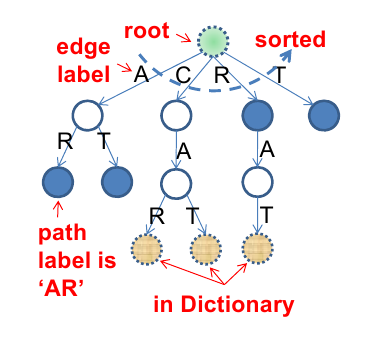
\includegraphics[width=.9\textwidth]{../img/suffixtrie_halim}\\
      % TODO: Replace suffix trie image with one of my own design
    \end{columns}
  }
\end{frame}

\begin{frame}
  \frametitle{Suffix Trie: Using it for a single, long string}
  {\smaller
  \begin{center}
    \structure{Suffix Trie (T='GATAGACA\alert{\$}')}
  \end{center}
  \begin{columns}[T]
    \column{0.35\textwidth}

    Create all $n$ suffixes:

    \begin{tabular}{c|l}
      i & suffix\\
      \hline
      0 & GATAGACA\$\\
      1 & ATAGACA\$\\
      2 & TAGACA\$\\
      3 & AGACA\$\\
      4 & GACA\$\\
      5 & ACA\$\\
      6 & CA\$\\
      7 & A\$\\
      8 & \$\\
    \end{tabular}

    Count the occurence of substring $m$:
    \begin{itemize}
    \item 'A': 4 times
    \item 'GA': 2 times
    \item 'AA': 0 times    
    \end{itemize}
    \column{0.65\textwidth}
    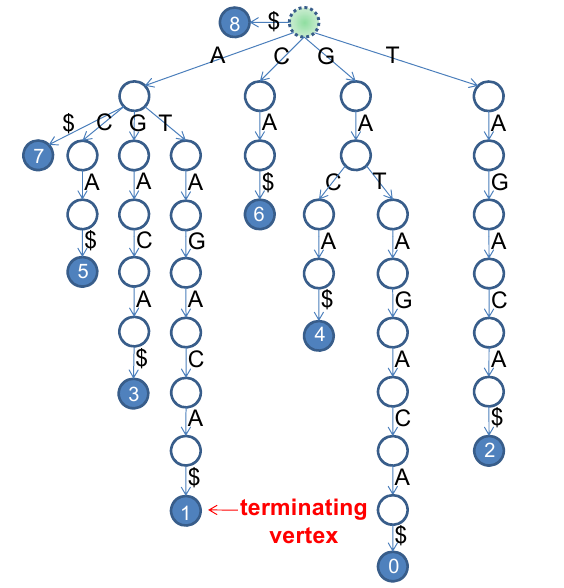
\includegraphics[width=.9\textwidth]{../img/suffixtrie_halim2}
  \end{columns}
  }
\end{frame}

\begin{frame}
  \frametitle{Suffix Trie: Suffix Tree}
  {\smaller
  \begin{center}
    \structure{Suffix Trie (T='GATAGACA\alert{\$}')}\\
    Compress single child nodes to obtain ``Suffix Tree''
  \end{center}
  \begin{columns}[T]
    \column{0.35\textwidth}

    \begin{tabular}{c|l}
      i & suffix\\
      \hline
      0 & GATAGACA\$\\
      1 & ATAGACA\$\\
      2 & TAGACA\$\\
      3 & AGACA\$\\
      4 & GACA\$\\
      5 & ACA\$\\
      6 & CA\$\\
      7 & A\$\\
      8 & \$\\
    \end{tabular}

    \bigskip

    With the suffix tree, many algorithms become faster.


    \column{0.65\textwidth}
    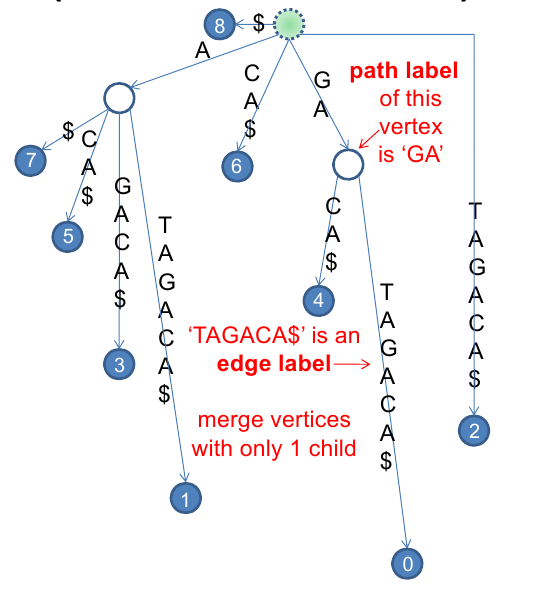
\includegraphics[width=.9\textwidth]{../img/suffixtree_halim}
  \end{columns}
  }
\end{frame}

\subsection{Uses of a Suffix Tree}
\begin{frame}
  \frametitle{Uses of a Suffix Tree 1: String Matching} {\smaller

    \structure{Assuming that we have the Suffix Tree already built},
    we can find all occurrences of substring $m$ in $T$ in time
    $O(m+\text{occ})$, where occ is the number of occurrences.

  \begin{center}
    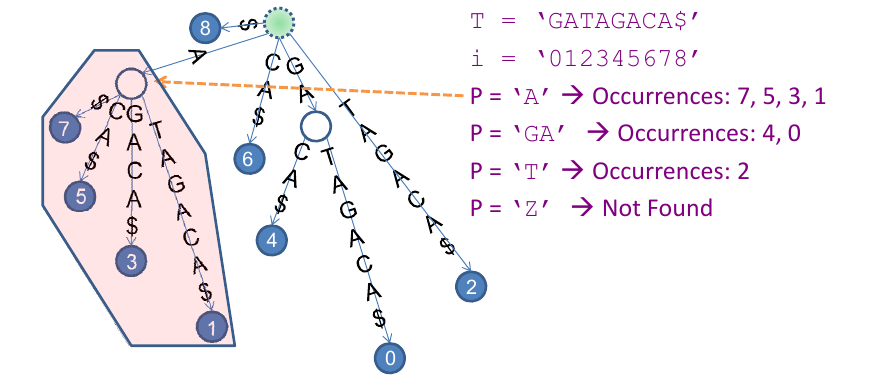
\includegraphics[width=0.9\textwidth]{../img/stringmatching_halim}
  \end{center}
  }
\end{frame}

\begin{frame}
  \frametitle{Uses of a Suffix Tree 2: Longest Repeated Substring}
  {\smaller
  \begin{itemize}
  \item The LRS is the longest substring with number of occurrences $> 2$;
  \item The LRS is the deepest internal node in the tree;
  \end{itemize}

  \begin{center}
    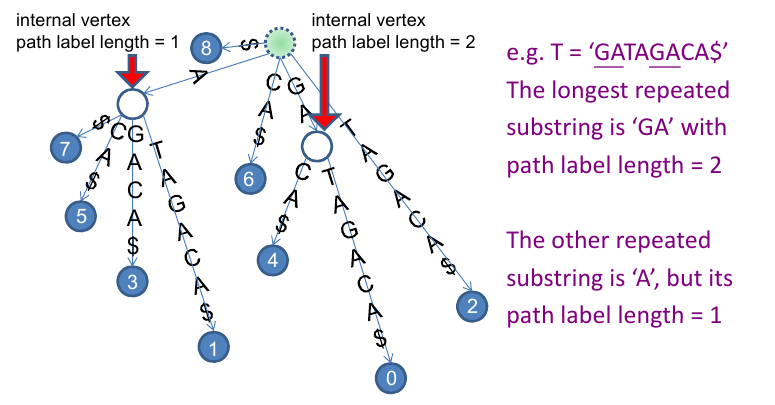
\includegraphics[width=0.9\textwidth]{../img/longestrepeatingsubstring_halim}
  \end{center}  
  }
\end{frame}

\begin{frame}
  \frametitle{Uses of a Suffix Tree 3: Longest Common Substring}
  {\smaller
    \begin{itemize}
    \item We can find the common substring of $M$ and $N$ by making a
      combined Suffix Tree. Each string has a different ending
      character.
    \item The common substring is the deepest node that has both characters.
    \end{itemize}
  \begin{center}
    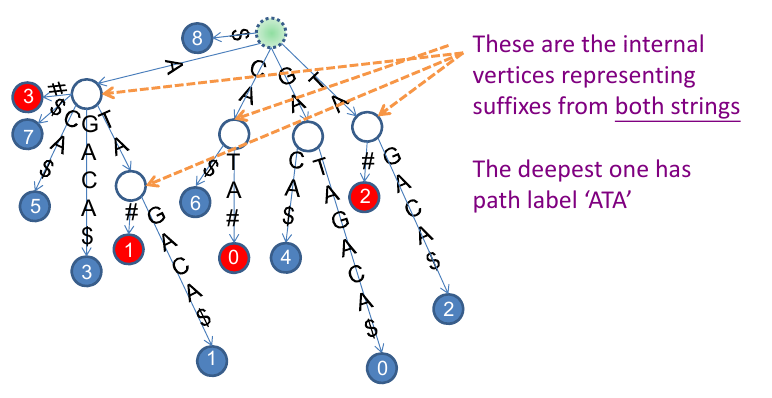
\includegraphics[width=0.9\textwidth]{../img/longestcommonsubstring_halim}
  \end{center}  
  }
\end{frame}

\subsection{Suffix Array}
\begin{frame}
  \frametitle{Suffix Trie: Suffix Array (1)}
  {\small
  \begin{itemize}
    \item The algorithms in previous slides are very efficient...\\
      ... \structure{if you have the suffix tree}

      \medskip

    \item The suffix tree can be built in $O(n)$...\\
      ... but implementation is rather complex;

      \medskip

    \item In this course, we will see the \structure{Suffix Array};

      \medskip

    \item The Suffix Array is built in $O(n\log{n})$...\\
      ... but the implementation is very simple!
  \end{itemize}

  \vfill

  \begin{block}{}
    I encourage you to study the implementation of the suffix tree by yourself!
  \end{block}
  }
\end{frame}

\begin{frame}
  \frametitle{Suffix Trie: Suffix Array (2)}

  {\smaller

    \begin{itemize}
    \item To make a Suffix array, make an array of all possible
      suffixes of $T$, and sort it;
    \item The order of the suffix array is the
      \structure{visit in preorder} of the suffix tree;
      % TODO: Japanese for pre-order visit
    \item We can adapt all algorithms accordingly;
    \end{itemize}

  \begin{columns}
    \column{0.4\textwidth}
    \begin{tabular}{c|l}
      i & suffix\\
      \hline
      0 & GATAGACA\$\\
      1 & ATAGACA\$\\
      2 & TAGACA\$\\
      3 & AGACA\$\\
      4 & GACA\$\\
      5 & ACA\$\\
      6 & CA\$\\
      7 & A\$\\
      8 & \$\\
    \end{tabular}
    \column{0.2\textwidth}
    Sort $\rightarrow$
    \column{0.4\textwidth}
    \begin{tabular}{c|c|l}
      i & SA[i] & suffix \\
      \hline
      0 & 8 & \$\\
      1 & 7 & A\$\\
      2 & 5 & ACA\$\\
      3 & 3 & AGACA\$\\
      4 & 1 & ATAGACA\$\\
      5 & 6 & CA\$\\
      6 & 4 & GACA\$\\
      7 & 0 & GATAGACA\$\\
      8 & 2 & TAGACA\$\\
    \end{tabular}
  \end{columns}
  }
\end{frame}

\begin{frame}[fragile,singleslide]
  \frametitle{Suffix Array: Implementation (1)}
  {\smaller
    \begin{exampleblock}{Simple Implementation}
\begin{verbatim}
#include <algorithm>
#include <cstdio>
#include <cstring>
using namespace std;
char T[MAX_N]; int SA[MAX_N],i,n;

bool cmp(int a, int b) { return strcmp(T+a, T+b) < 0; } 
// O(n)

int main() {
  n = (int) strlen (gets(T));
  for (int i = 0; i < n; i++) SA[i] = i;
  sort (SA, SA+n, cmp); // O(n^2 log n) }
\end{verbatim}
    \end{exampleblock}

    This implementation is too slow for strings bigger than 1000 characters.
  }
\end{frame}

\begin{frame}[fragile,singleslide]
  \frametitle{Suffix Array: Implementation (2.1)}
  {\smaller
    \begin{exampleblock}{O(n log n) implementation using ``ranking pairs/radix sort''}
\begin{verbatim}
char T[MAX_N]; int n; int c[MAX_N]; 
int RA[MAX_N], tempRA[MAX_N], SA[MAX_N], tempSA[MAX_N];

void countingSort(int k) {
  int i, sum, maxi = max(300,n); //255 ASCII chars or n
  memset(c, 0, sizeof(c));
  for (i = 0; i < n; i++) c[i+k<n? RA[i+k] : 0]++
  for (i = sum = 0; i < maxi; i++) 
    { int t = c[i]; c[i] = sum; sum += t;} //frequency
  for (i = 0; i < n; i++)
    tempSA[c[SA[i]+k < n ? RA[SA[i]+k] : 0]++] = SA[i];
  for (i = 0; i < n; i++) // update suffix array
    SA[i] = tempSA[i];
}

// ... continues next slide
\end{verbatim}
    \end{exampleblock}
  }
\end{frame}

\begin{frame}[fragile,singleslide]
  \frametitle{Suffix Array: Implementation (2.2)}
  {\smaller
    \begin{exampleblock}{O(n log n) implementation using ``ranking pairs/radix sort''}
\begin{verbatim}
// ... continued from last slide

void constructSA() {
  int i, k, r;
  for (i = 0; i < n; i++) { RA[i] = T[i]; SA[i] = i;}
  for (k = 1; k < n; k <<=1) {
    countingSort(k); countingSort(0);
    tempRA[SA[0]] = r = 0;
    for (i = 1; i < n; i++) tempRA[SA[i]] = 
           (RA[SA[i]] == RA[SA[i-1]] && 
            RA[SA[i]+k] == RA[SA[i-1]+k]) ? r : ++r;
    for (i = 0; i < n; i++)
      RA[i] = tempRA[i];
    if (RA[SA[n-1]] == n-1) break;
}}
\end{verbatim}
    \end{exampleblock}
  }
\end{frame}

\begin{frame}
  \frametitle{Suffix Array: Using Suffix Array (1)}
  {\smaller
    \begin{block}{String Matching: Finding 'GA'}
      \begin{itemize}
      \item Do a binary search once to find the lower bound;
      \item Do a binary search once to fint the upper bound;
      \end{itemize}
    \end{block}
    \begin{center}
      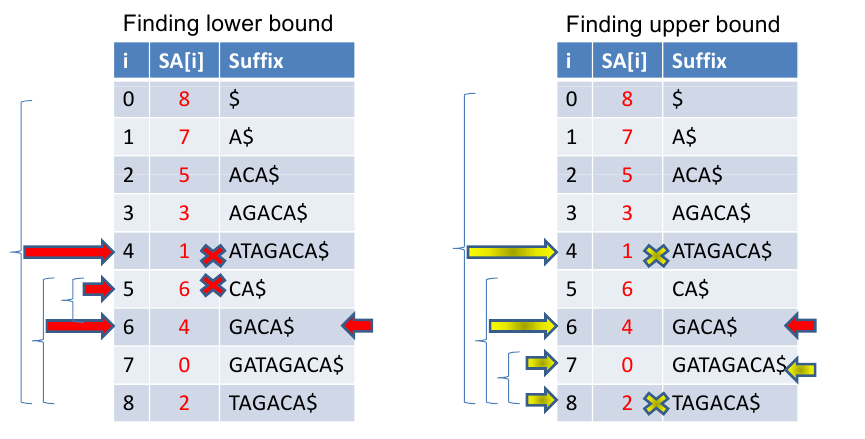
\includegraphics[width=0.9\textwidth]{../img/suffixarray_halim}
    \end{center}
  }
\end{frame}

\begin{frame}
    \frametitle{Suffix Array: Using Suffix Array (2)}
  {\smaller
    \begin{block}{Longest Repeated Substring}
      Find the longest common prefix between suffix $i$ and $i+1$
    \end{block}
    \begin{center}
      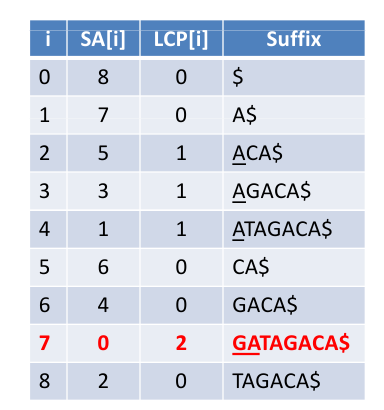
\includegraphics[width=0.5\textwidth]{../img/suffixarray2_halim}
    \end{center}
  }
\end{frame}

\begin{frame}
    \frametitle{Suffix Array: Using Suffix Array (3)}
  {\smaller
    \begin{block}{Longest Common Substring}
      \begin{itemize}
      \item Create Suffix Array for appended strings $MN$;
      \item Find the longest common prefix that has both string enders;
      \end{itemize}
    \end{block}
    \begin{center}
      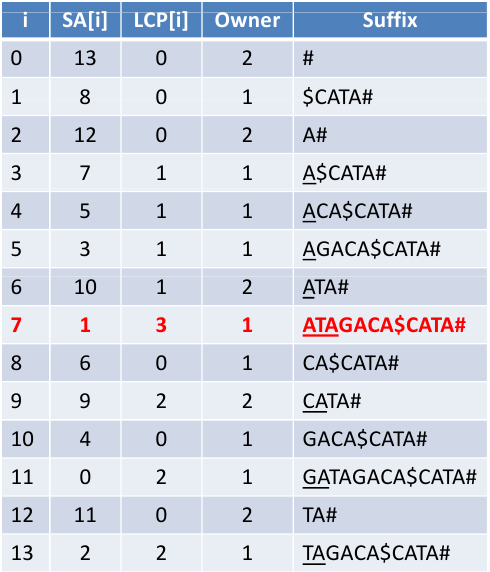
\includegraphics[width=0.45\textwidth]{../img/suffixarray3_halim}
    \end{center}
  }
\end{frame}

\section{Conclusion}

\subsection{Problem Discussion}
\begin{frame}
  \frametitle{Problem Discussion}
  \begin{itemize}
  \item Immediate Decodability
  \item Caesar Cypher
  \item Ensuring Truth
  \item Smeech
  \item String Partition
  \item Prince and Princess
  \item Power Strings
  \item Life Forms
  \end{itemize}
\end{frame}

\begin{frame}
  \frametitle{Final Message}
  \begin{center}
    Thank you for participating in this class!\\
    I hope your programming abilities have improved!

    \vfill

    Remember: Your brain is like a muscle, it needs constant practice to keep itself smart
  \end{center}
\end{frame}

\end{document}

